\subsection{Organisation du travail}
\label{section:eyrolles_organisation}

Pour ma part, j'ai été affecté en tant que développeur sur le projet \aey. J'ai pu travailler avec \acohen, le chef de projet, ainsi que les développeurs \ahamon, \aweistroff\ et \abachelet. 

Cette section décrit les différentes phases du projet \aey\ et reprend son planning.


\subsubsection{Planning}

Le planning tel qu'il a été établi au début du projet est le suivant :

\begin{description}
	\item[Phase de développement] du 21 septembre 2009 au 11 décembre 2009 ;
	\item[Phase de recette] du 14 décembre 2009 au 8 janvier 2010 ;
	\item[Livraison finale] le 11 janvier 2010.
\end{description}

Le planning réel a pris du retard sur le planning initial :

\begin{description}
	\item[Phase de développement] du 21 septembre 2009 au 11 décembre 2009 ;
	\item[Phase de recette] du 14 décembre 2009 au 17 février 2010 ;
	\item[Livraison finale] le 18 février 2010.
\end{description}

Note : les phases de spécification et d'analyse ne sont pas listées dans le planning du fait que je n'étais pas encore arrivé chez \asl\ quand elles ont eu lieu.


\subsubsection{Phase de spécification}

Conjointement avec le client, \acohen\ s'est chargé de la rédaction du cahier des charges du projet. Il en ressort un dossier d'une centaine de pages, décrivant les fonctionnalités attendues, les règles métiers ou encore des prototypes d'interface utilisateur. C'est ce document qui a servi de fil rouge tout au long de la réalisation du projet.


\subsubsection{Phase d'analyse}

La phase d'analyse du projet a consisté à mettre en place le modèle de l'application sous la forme d'un diagramme, le \amcd\footnote{Le \amcd, ou Modèle Conceptuel de Données, établit sous forme de diagramme une représentation des données et définit les dépendances fonctionnelles entre elles.}. À l'\autc, nous avons eu l'occasion de réaliser des \amcds\ dans l'\auv\ NF17\footnote{Cours de conception de bases de données à l'\autc.} en utilisant le format \auml\footnote{\auml\ (\textit{Unified Modeling Language}) est un langage de modélisation graphique standardisé utilisé dans le domaine du génie logiciel, notamment dans le cadre de la conception orientée objet.~\cite{uml}} ou \aea\footnote{Le modèle entité-association, ou modèle \aea, est une représentation abstraite et et conceptuelle de données. Il est notamment utilisé pour modéliser des schémas de base de données.~\cite{ea}}. Chez \asl, les diagrammes \amcds\ sont réalisés au format \aea\ et sont réalisés à l'aide de l'outil \amysqlwb.

Le \amcd\ du \alotdeux\ d'\aey, modélisé par \acohen\ et \ahamon, comprend de nombreuses tables et de nombreux liens. Pour gagner en lisibilité, les tables et les liens n'ont pas tous été représentés : seuls les plus importants permettant de mieux comprendre le fonctionnement de l'application ont été choisis.


\subsubsection{Phase de développement}

Ma participation au projet \aey\ a commencé au début de la phase de développement. Avec \ahamon, nous y avons développé la plupart des fonctionnalités attendues\footnote{Cf. section~\ref{section:eyrolles_fct}}. Début décembre, \aweistroff, qui venait d'être embauché par \asl, nous a rejoint pour soutenir le rythme d'implémentation.

La répartition du travail s'est mise en place simplement en affectant, au fur et à mesure de l'avancement du projet, une fonctionnalité à implémenter à chaque développeur. Chaque fonctionnalité à traiter a été choisie par le chef de projet en fonction de sa priorité estimée. Le code source de l'application était partagé via un dépôt \asvn\footnote{Cf. section~\ref{section:outils_svn}}.

Le \alotdeux\ de l'\aintranet\ d'\aey\ utilise la version 1.3 de \asf. Au moment où le développement du projet avait commencé, cette version du \afm\ n'était pas encore sortie en version finale et était encore en plein développement. Comme c'est \asl\ qui est à l'origine de \asf, la maîtrise sur le \afm\ en interne est importante : l'entreprise peut donc se permettre d'utiliser les dernières technologies disponibles.

Les contraintes techniques de développement imposent d'utiliser une base de données \apsql, à la demande du client. L'utilisation de \asf\ 1.3, quant à elle, nécessite une version de \aphp\ supérieure à 5.2.4. Le serveur \ahttp\ utilisé est \aapache~2.


\subsubsection{Phase de recette}
\label{section:eyrolles_organisation_recette}

La phase de recette consiste à faire tester l'application au client, qui va pouvoir faire remonter les éventuels \abugs\ à corriger ou les fonctionnalités à améliorer. La communication entre le client, le chef de projet et les dé\-ve\-lop\-peurs s'est déroulée via le système de gestion de projet \atrac\footnote{Cf. section~\ref{section:outils_trac}}.

En fait, le client y rédige la description de son \abug\ dans un ticket. Le chef de projet le valide, et l'assigne ensuite au développeur qui doit s'en charger. Une fois que le développeur a fait son travail d'implémentation sur un ticket, il le renvoie au chef de projet qui vérifie la fonctionnalité modifiée. Si tout se passe bien, le ticket est retourné à nouveau au client pour qu'il se rende compte par lui-même de l'amélioration. Le client satisfait clôt alors le ticket ; dans le cas contraire, il initie un nouveau cycle d'échange sur celui-ci. Ce processus de recette via rapports de \abugs\ est illustré dans la figure~\ref{figure:eyrolles_organisation_tickets}.

\begin{figure}
	\centering
	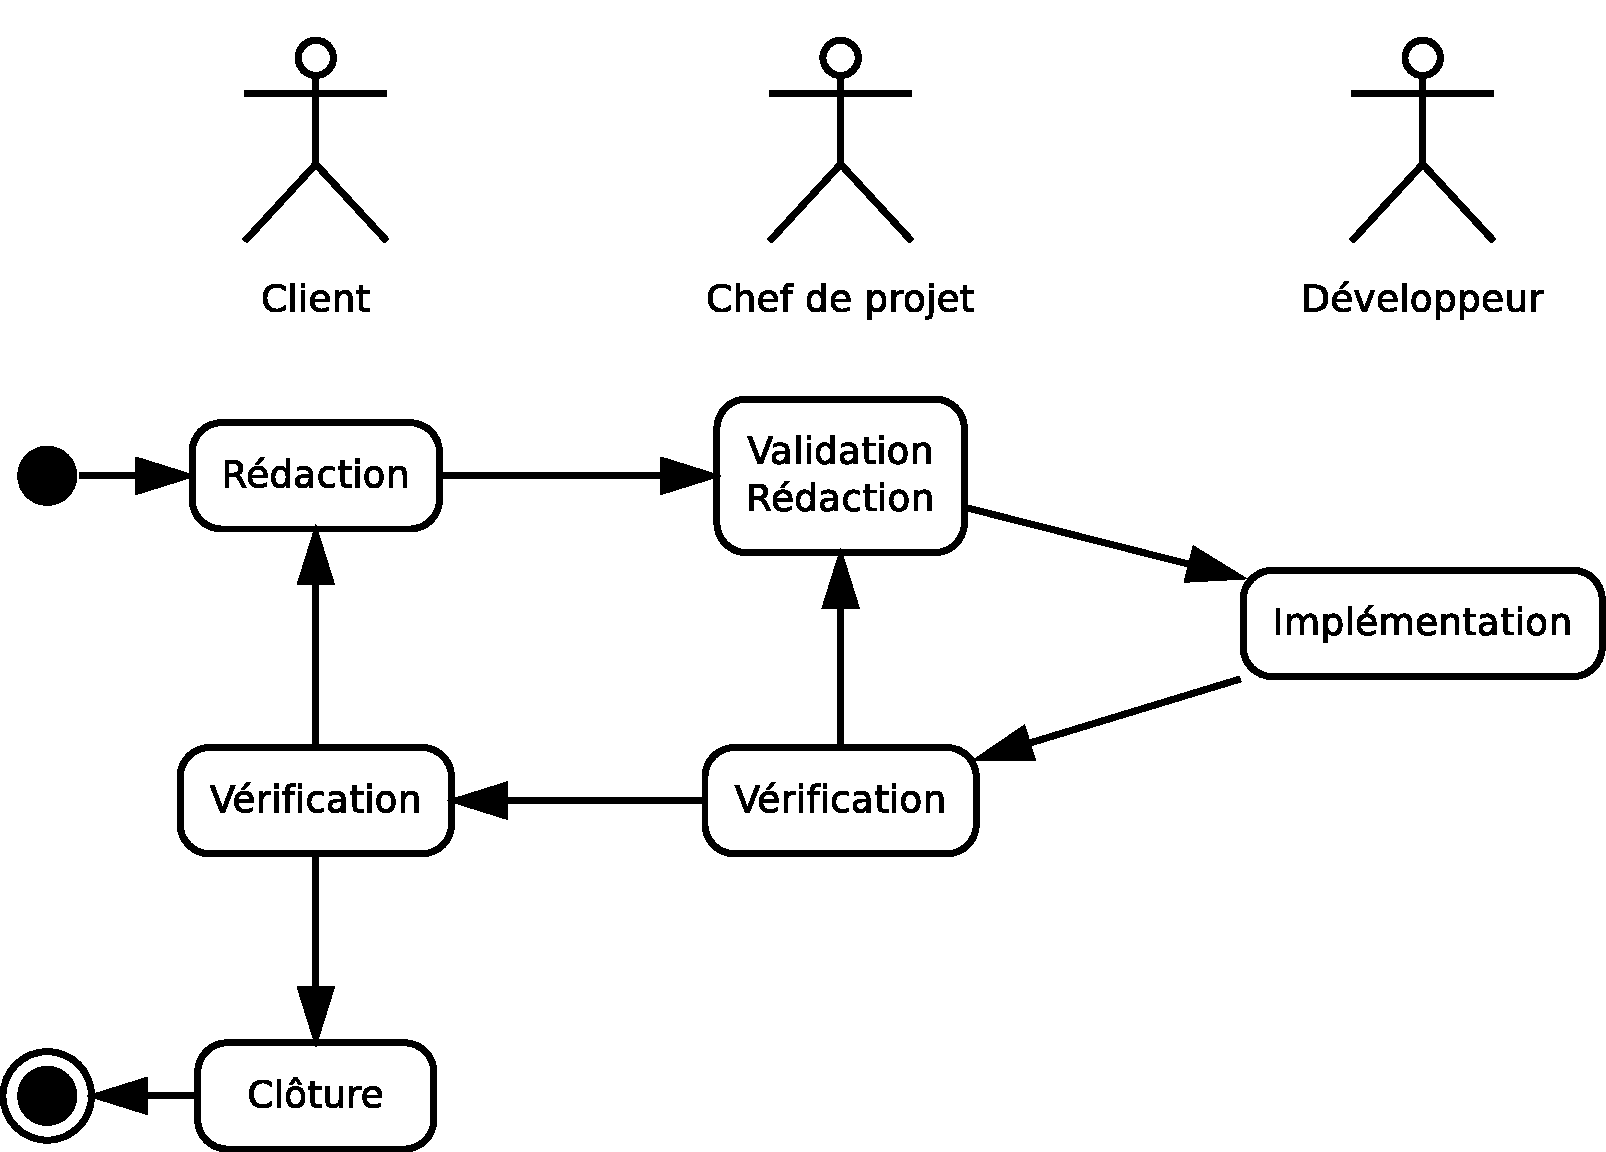
\includegraphics[scale=0.4]{eyrolles_organisation_tickets}
	\caption{États d'un ticket dans le cas du processus de recette d'\aey}
	\label{figure:eyrolles_organisation_tickets}
\end{figure}

Par ailleurs, pour permettre au client de tester correctement l'application, il est nécessaire de lui montrer régulièrement les nouvelles versions du projet. Cette démarche s'est traduite par une livraison hebdomadaire de l'application sur le serveur du client. Le processus de livraison d'\aey\ est décrit plus tard dans la section~\ref{section:eyrolles_prod}.

Du point de vue de l'organisation du travail, \ahamon\ a quitté l'équipe de développement d'\aey\ au moment du passage en phase de recette, afin de s'occuper du pôle formation de \asl. Pendant trois semaines, j'ai continué avec \aweistroff, qui a ensuite été affecté sur un autre projet début janvier. J'ai continué pendant quelques temps à développer seul sur le projet, et fin janvier, \abachelet\ m'a rejoint ponctuellement pour m'aider à fermer les tickets restants.

Comme le montre le planning réel, c'est cette phase qui a pris du retard. Le premier facteur correspond au fait que nous avons passé l'application en recette alors qu'il restait encore quelques fonctionnalités à développer. Le second, quant à lui, est issu de changements structurels importants, apportés au dernier moment durant la phase précédente, qui ont engendré bon nombre de \abugs.


\subsubsection{Livraison finale}

La livraison finale ayant été repoussée après mon départ, je n'aurais pas eu l'occasion d'y participer. Toutefois, le processus sera exactement le même que celui utilisé durant la phase de recette.
